\documentclass{article}

% Language setting
% Replace `english' with e.g. `spanish' to change the document language
\usepackage[english]{babel}

% Set page size and margins
% Replace `letterpaper' with `a4paper' for UK/EU standard size
\usepackage[letterpaper,top=2cm,bottom=2cm,left=3cm,right=3cm,marginparwidth=1.75cm]{geometry}
\usepackage{CJKutf8}
% Useful packages
\usepackage{amsmath}
\usepackage{graphicx}
\usepackage{setspace}
\usepackage{float}
\usepackage{subfigure}
\usepackage[section]{placeins}
\usepackage[colorlinks=true, allcolors=blue]{hyperref}
\usepackage[export]{adjustbox}

\author{B10209040 陳彥倫}

\begin{document}
\thispagestyle{empty}
\hfill {\scshape \large Statistics with Meteorological Applications, Spring 2024} \hfill {\scshape P1}
\smallskip
\hrule
\begin{CJK*}{UTF8}{bsmi}
\bigskip
\bigskip
\bigskip

\centerline{\huge \textbf {HW1}}
\bigskip
\centerline{\textbf {B10209040 陳彥倫}}

\section*{a.}
\begin{spacing}{2}
    \begin{large}

    \end{large}
\end{spacing}

\begin{figure}[htbp]
    \centering
    \begin{minipage}[t]{0.48\textwidth}
        \centering
        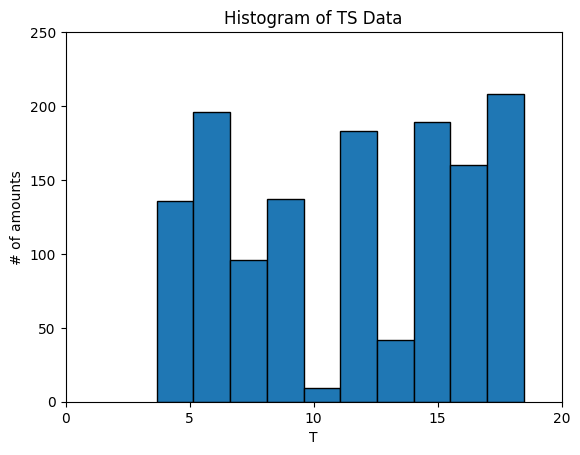
\includegraphics[width=6cm]{1.png}
        \caption{original}
        \end{minipage}
    \begin{minipage}[t]{0.48\textwidth}
        \centering
        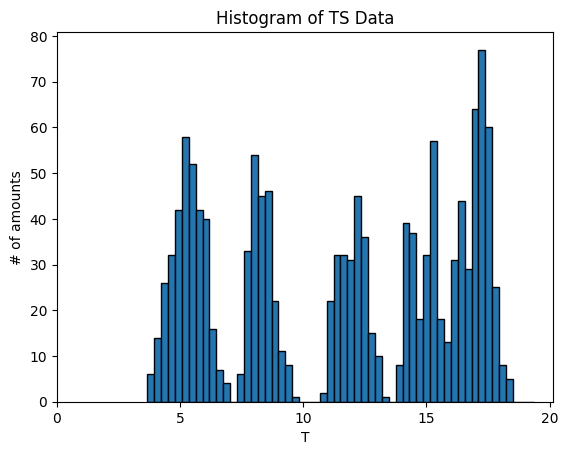
\includegraphics[width=6cm]{2.png}
        \caption{After adjusting the bins}
        \end{minipage}
    \begin{minipage}[t]{0.48\textwidth}
        \centering
        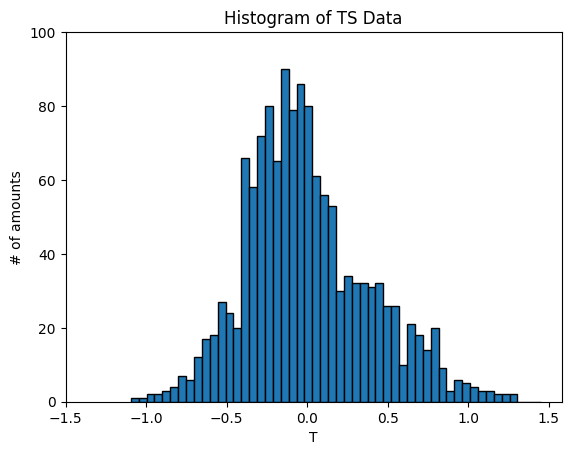
\includegraphics[width=6cm]{3.png}
        \caption{After removing the seasonal cycle}
        \end{minipage}
\end{figure}

\subsection*{Discussion}
\begin{spacing}{2}
    \begin{large}
        以x軸為surface temperature,y軸為出現次數做成直方圖統計,可以得到Figure 1之結果
        ,但無法觀察出如一般數據點類似於常態分佈的pattern。若將x軸的間隔縮小,則可以觀察出數
        個由低溫到高溫排列、因季節變化造成的常態分佈。計算出季節週期後相減得到較合理的圖形分布。
    \end{large}
\end{spacing}

\newpage

\thispagestyle{empty}
\hfill {\scshape \large Statistics with Meteorological Applications, Spring 2024} \hfill {\scshape P2}
\smallskip
\hrule
\bigskip
\bigskip
\bigskip

\section*{b.}
\begin{spacing}{2}
    \begin{large}
        有一實驗設計藉由告知各藥物的臨床成功率以及個案的情況來統計人們對這些藥物的接受度,
        結果發現只要該個案情況不佳的那種藥物接收度皆極低,由此可以得知個案為影響大眾心理的
        重要因素之一。這可能是因為我們本能上可以理解他人的實際經驗,但實驗數據如臨床成功率
        之類之名詞概念則需靠學習以更進一步的解讀,而這並不是每個人都能做到或接受的。適當運
        用數據及個案實例來佐證自己的論點及想法才是上策。
    \end{large}
\end{spacing}







\end{CJK*}
\end{document}